%
% latex template for SRS documentation 
% name: srs.tex 
% date last modified: 25 feb 2018
% modified by: guru 
% 
%
\documentclass{article}

\usepackage{caption}
\usepackage[margin=1in]{geometry}
\usepackage{graphicx}
\usepackage{hyperref}
\usepackage{float}
\usepackage{tabularx}
\usepackage{titling}

\begin{document}

\title{
	CSC431 \\
	\vspace{0.2in}
	\textbf{Download of Public-facing Data} \\
	\large Software Requirements Specification \\
	Team \#3
}

\author{
	Jerry Bonnell
	\and Gururaj Shriram
	\and Erica Chang
	\and Heyu Yao
	\and Lixiong Liang
}

\date{}
\maketitle

\clearpage
\section*{Version History}

\begin{tabularx}{\textwidth}{| l | l | X | X |}
	\hline
	\textbf{Version} & \textbf{Date} & \textbf{Author(s)} & \textbf{Change Comments} \\
	\hline
	1                & \today        & xxx                & xxx                      \\
	\hline
	                 &               &                    &                          \\
	\hline
	                 &               &                    &                          \\
	\hline
\end{tabularx}

\clearpage
\tableofcontents

\clearpage
\listoffigures
\listoftables

\clearpage

\section{System Requirements}

\subsection{Functional Requirements}

\subsubsection{Download of Public-facing Data}

\begin{table}[H]
	\caption{Download of Public-facing Data}
	\begin{tabularx}{\textwidth}{|l|X|}
		\hline
		\textbf{Title}            & Download of Public-facing Data            \\ \hline
		\textbf{Description}      & User can choose an output format for
		queried data and download locally to computer. \\ \hline
		\textbf{Source Scenario}  & FR1                                       \\ \hline
		\textbf{Priority}         & Mandatory: 0                              \\ \hline
		\textbf{Precondition(s)}  & List of layers consisting of cadastral,
		multimedia, and workshop data is passed to the server. Output format
		is given: one of \texttt{GeoJSON}, esri \texttt{shapefile}, \texttt{kml},
		or \texttt{CSV} \\ \hline
		\textbf{Postcondition(s)} & Data is packaged into a zip file and sent
		back to the browser for local download. \\ \hline
		\textbf{Use Case Diagram} &                                           \\  \hline
	\end{tabularx}
\end{table}

\subsection{Non-Functional Requirements}

\subsubsection{Minimum Simultaneous Downloads}

\begin{table}[H]
	\caption{Minimum Simultaneous Downloads}
	\begin{tabularx}{\textwidth}{|l|X|}
		\hline
		\textbf{Title}            & Minimum Simultaneous Downloads          \\ \hline
		\textbf{Description}      & The download server must handle up to 3
		simultaneous download requests. \\ \hline
		\textbf{Source Scenario}  & NFR1                                    \\ \hline
		\textbf{Priority}         & High: 1                                 \\ \hline
		\textbf{Applicable FR(s)} & FR1                                     \\ \hline
	\end{tabularx}
\end{table}

\pagebreak

\section{System Constraints}

\subsection{Tool Constraints}

\subsubsection{Web Application Framework Constraint}

\textbf{References:}
\begin{itemize}
	\item \url{https://nodejs.org}
	\item \url{https://expressjs.com/}
\end{itemize}

\begin{table}[H]
	\caption{Web Application Framework Constraint}
	\begin{tabularx}{\textwidth}{|l|X|}
		\hline
		\textbf{Title}       & Web Application Framework Constraint              \\ \hline
		\textbf{Description} & We will be using Express/Node.js as the framework
		for the backend. This will allow for greater ease of deployment on the
		server-side. \\ \hline
		\textbf{Priority}    & Mandatory: 0                                      \\ \hline
	\end{tabularx}
\end{table}

\begin{table}[H]
	\caption{geojson2 Conversion Package}
	\begin{tabularx}{\textwidth}{|l|X|}
		\hline
		\textbf{Title}       & geojson2 Conversion Package             \\ \hline
		\textbf{Description} & We will be using geojson2 which is a geojson exporting utility belt that can convert a geojson object into several other formats. This package uses the ogr2ogr node package to perform the conversions.      \\ \hline
		\textbf{Priority}    & Mandatory: 0 \\ \hline
	\end{tabularx}
\end{table}

\begin{table}[H]
	\caption{Archiver Packaging Tool}
	\begin{tabularx}{\textwidth}{|l|X|}
		\hline
		\textbf{Title}       & Archiver Packaging Tool                  \\ \hline
		\textbf{Description} & We will use the Archiver node module in order to package all of the requested files into a zip or tar file.      \\ \hline
		\textbf{Priority}    & High: 2 \\ \hline
	\end{tabularx}
\end{table}

\subsection{Language Constraints}

\subsubsection{Backend REST Framework}

\begin{table}[H]
	\caption{Backend REST Framework}
	\begin{tabularx}{\textwidth}{|l|X|}
		\hline
		\textbf{Title}       & Backend REST Framework                      \\ \hline
		\textbf{Description} & Because we are using the Express framework,
		Javascript is a requirement. Therefore, the backend will be written
		in Javascript. \\ \hline
		\textbf{Priority}    & Mandatory: 0                                \\ \hline
	\end{tabularx}
\end{table}

\subsection{Platform Constraints}

\subsubsection{Web Service Platform}

\begin{table}[H]
	\caption{Web Service Platform}
	\begin{tabularx}{\textwidth}{|l|X|}
		\hline
		\textbf{Title}       & Web Service Platform                      \\ \hline
		\textbf{Description} & Express/Node.js is, fortunately, platform
		independent. Further, a platform constraint has not been set by the
		client for this team.       \\ \hline
		\textbf{Priority}    & Lowest: 5                                 \\ \hline
	\end{tabularx}
\end{table}

\subsection{Hardware Constraints}

As we are using Amazon EC2 for deployment, our hardware constraints are set by the free-tier package Amazon provides. \\

\textbf{References:}
\begin{itemize}
	\item \url{https://aws.amazon.com/ec2/}
\end{itemize}

\subsubsection{Storage Constraints}

\begin{table}[H]
	\caption{Storage Constraints}
	\begin{tabularx}{\textwidth}{|l|X|}
		\hline
		\textbf{Title}       & Storage Constraints                          \\ \hline
		\textbf{Description} & Our storage constraint is set by Amazon EC2.
		However, storage constraints are of minimal priority for this team
		as there will be nothing stored on disk.        \\ \hline
		\textbf{Priority}    & Lowest: 5                                    \\ \hline
	\end{tabularx}
\end{table}

\subsubsection{Computation Constraints}

\begin{table}[H]
	\caption{Computation Constraints}
	\begin{tabularx}{\textwidth}{|l|X|}
		\hline
		\textbf{Title}       & Computation Constraints                          \\ \hline
		\textbf{Description} & Our computation constraint is also set by Amazon
		EC2. Its free-tier service is ample for this team as our service
		primarily converts and packages data.          \\ \hline
		\textbf{Priority}    & Low: 4                                           \\ \hline
	\end{tabularx}
\end{table}

\subsection{Network Constraints}

\subsubsection{Access Database}

\begin{table}[H]
	\caption{Access Database}
	\begin{tabularx}{\textwidth}{|l|X|}
		\hline
		\textbf{Title}       & Access Database                              \\ \hline
		\textbf{Description} & Our service must be able to query a PostGRES
		database over the network in order to fetch geospatial and multimedia
		data.     \\ \hline
		\textbf{Priority}    & Mandatory: 0                                 \\ \hline
	\end{tabularx}
\end{table}

\subsubsection{Download Response}

\begin{table}[H]
	\caption{Download Response}
	\begin{tabularx}{\textwidth}{|l|X|}
		\hline
		\textbf{Title}       & Download Response                                 \\ \hline
		\textbf{Description} & Our service must be able to package and send back
		data to the browser over HTTP protocol for local download. \\ \hline
		\textbf{Priority}    & Mandatory: 0                                      \\ \hline
	\end{tabularx}
\end{table}

\subsection{Deployment Constraints}

\subsubsection{AWS EC2 Deployment}

\begin{table}[H]
	\caption{AWS EC2 Deployment}
	\begin{tabularx}{\textwidth}{|l|X|}
		\hline
		\textbf{Title}       & AWS EC2 Deployment                              \\ \hline
		\textbf{Description} & The web service will be deployed on Amazon EC2.
		Amazon provides a free-tier service for 12 months that will last the
		duration of the semester.        \\ \hline
		\textbf{Priority}    & Medium: 3                                       \\ \hline
	\end{tabularx}
\end{table}

\subsection{Transition \& Support Constraints}

\subsubsection{Transitionary Requirements}

\begin{table}[H]
	\caption{Transitionary Requirements}
	\begin{tabularx}{\textwidth}{|l|X|}
		\hline
		\textbf{Title}       & Transitionary Requirements             \\ \hline
		\textbf{Description} & Once the user selects the needed data elements and desired file format, our service must download the data and package it in a convenient manner for the user.      \\ \hline
		\textbf{Priority}    & Mandatory: 0 \\ \hline
	\end{tabularx}
\end{table}

\subsection{Budget \& Schedule Constraints}

\subsubsection{Time Constraints}

\begin{table}[H]
	\caption{Time Constraints}
	\begin{tabularx}{\textwidth}{|l|X|}
		\hline
		\textbf{Title}       & Time Constraints                           \\ \hline
		\textbf{Description} & The service must be designed and developed before May 7, 2018      \\ \hline
		\textbf{Priority}    & Mandatory: 0 \\ \hline
	\end{tabularx}
\end{table}

\subsection{Miscellaneous Constraints}

\subsubsection{Performance Constraints}

\begin{table}[H]
	\caption{Performance Constraints}
	\begin{tabularx}{\textwidth}{|l|X|}
		\hline
		\textbf{Title}       & Performance Constraints                           \\ \hline
		\textbf{Description} & The speed and quality of the service is directly dependent on the reliability of the Search results and the access database's schema.      \\ \hline
		\textbf{Priority}    & Low: 4 \\ \hline
	\end{tabularx}
\end{table}

\clearpage

\section{Requirements Modeling}

\subsection{Download Public-Facing Data}

\begin{figure}[H]
	\begin{center}
		\caption{Download Public-Facing Data}
		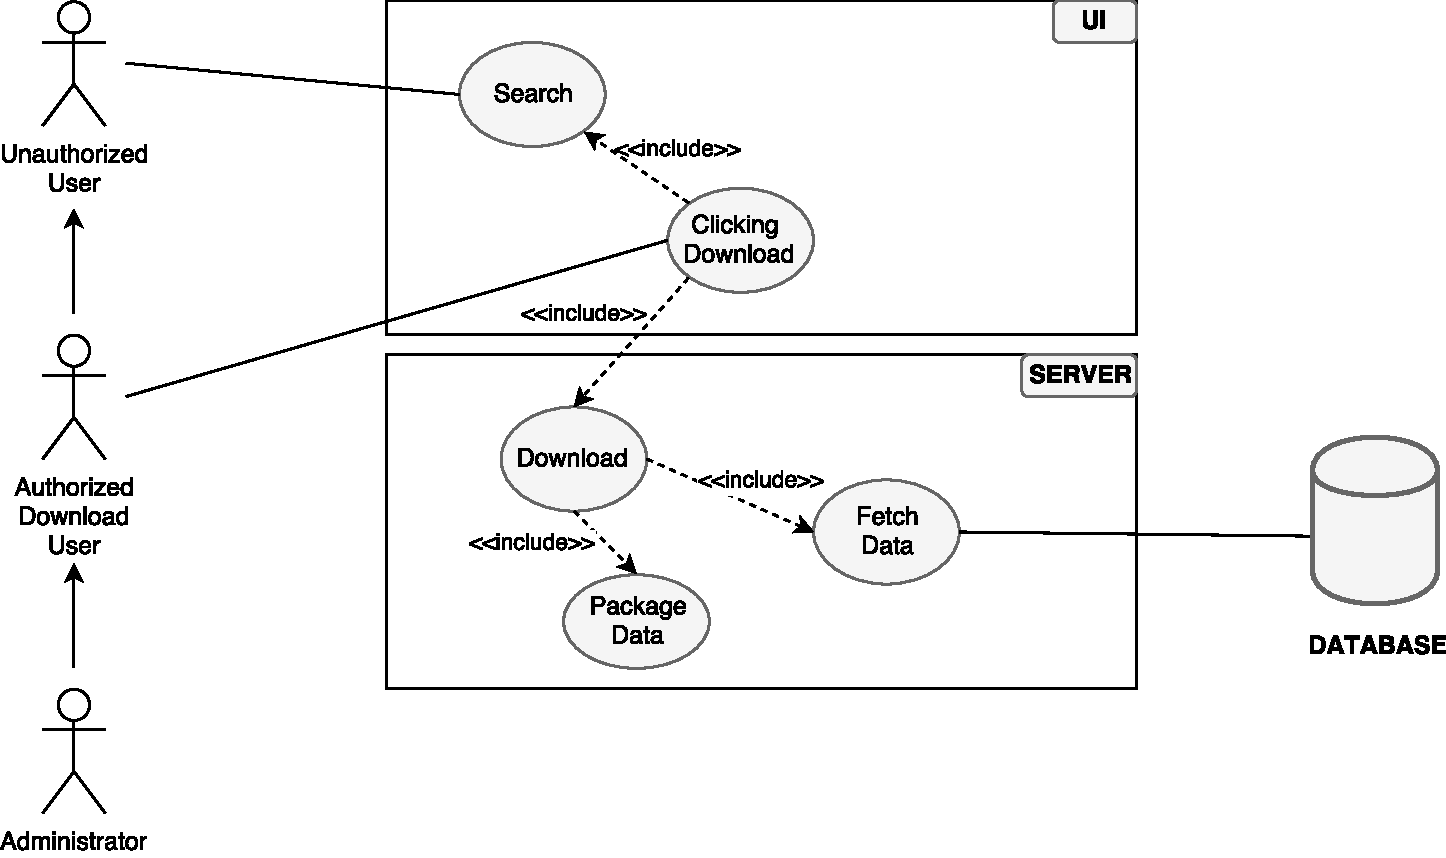
\includegraphics[width=\textwidth]{images/download-use-case.pdf}
	\end{center}
\end{figure}

\clearpage

\section{Evolutionary Requirements (TBA in further iterations of the SRS)}

\subsection{Functional Requirements}

\subsubsection{Requirement Title}

\begin{table}[H]
	\caption{Table title}
	\begin{tabularx}{\textwidth}{|l|X|}
		\hline
		\textbf{Title}            & Insert title                           \\ \hline
		\textbf{Description}      & A one or two sentence description      \\ \hline
		\textbf{Priority}         & Priority from 0 (highest) - 5 (lowest) \\ \hline
		\textbf{Precondition(s)}  & What needs to happen before            \\ \hline
		\textbf{Postcondition(s)} & What happens as a result               \\ \hline
		\textbf{Use Case Diagram} & Link or number, if present             \\  \hline
	\end{tabularx}
\end{table}

\subsection{Functional Requirements}

\subsubsection{Requirement Title}

\begin{table}[H]
	\caption{Table title}
	\begin{tabularx}{\textwidth}{|l|X|}
		\hline
		\textbf{Title}            & Insert title                                          \\ \hline
		\textbf{Description}      & A one or two sentence description                     \\ \hline
		\textbf{Priority}         & Priority from 0 (highest) - 5 (lowest)                \\ \hline
		\textbf{Applicable FR(s)} & What functional requirement(s) is this applicable to? \\ \hline
	\end{tabularx}
\end{table}


\end{document}